\documentclass[a4paper,10pt]{article}

\usepackage{amsmath}
\usepackage{amssymb}
\usepackage{amsthm}
\usepackage{charter}
\usepackage{color}
\usepackage{graphicx}
\usepackage{hyperref}
\usepackage[utf8]{inputenc}
\usepackage{listings}
\usepackage{url}

\definecolor{grey}{rgb}{0.9,0.9,0.9}

\lstset{
language=Python,
basicstyle=\footnotesize\fontfamily{pcr},
backgroundcolor=\color{grey},
numbers=left,
numberstyle=\tiny,
numbersep=5pt,
showstringspaces=false,
tabsize=2,
breaklines=true
}

\setlength{\parindent}{0pt}

%opening
\sloppy

\newcommand{\dbf}[1]{\operatorname{dbf}(#1)}

\newtheorem{definition}{Definition}
\newtheorem{theorem}{Theorem}

\newtheorem*{remarks}{Remarks}

\begin{document}

\title{Using DIT to simplify the DBF feasibility test}
\author{Thomas Chapeaux \\ ~ \\ \emph{Supervisor} \\ Laurent George, ECE Paris \\ ~ \\ \emph{Thanks to} \\ Paul Rodriguez}

\date{July 2013}

\maketitle

\tableofcontents

\newpage

\section{Real-Time Systems}

$\tau = \{ \tau_1, \cdots, \tau_n \}$

$\tau_i = (O_i, C_i, D_i, T_i)$

$H = LCM(T_i)$

\begin{definition}
	A system is \textbf{synchronous} if all its tasks have no offset, and
	\textbf{asynchronous} otherwise.
\end{definition}

\section{The DBF feasibility test}
\label{sct:DBF}

\subsection{Definition of the demand-bound function}

\begin{definition}
 The \textbf{demand-bound function (DBF)}
 \cite{baruah1999generalized, baruah1990algorithms} defined for a task set
 $\tau$ and noted $\dbf{t}$, is equal to the maximal cumulated execution time of jobs of $\tau$ contained in any interval of length $t$.\\

 Mathematically,
 $$\dbf{t} = \max_{\{\forall \: t_1, t_2 \mid t_2 - t_1 = t \: \wedge \: 0
 \leqslant t_1 \leqslant t_2\}} \sum_{i=1}^n C_i \cdot h_i(t_1, t_2)$$ where
 $h_i(t_1, t_2)$ is the number of jobs of task $i$ whose arrival and deadline are in (non-strict) the interval $[t_1, t_2]$.
\end{definition}

As the synchronous arrival pattern is known to be the worst case
\cite{liu1973scheduling}, in that particular case we can only consider the
interval $[0, t]$. In an asynchronous arrival pattern, it is sufficient to check
only intervals where $t_2 < O_{max} + 2H$, as the system will be
periodic starting from $O_{max} + H$ or sooner \cite{leung1982complexity}.\\

In the sequel a closed form expression of the DBF is given in the synchronous
case. Intuitively, in this case it will be a step-function whose increases will
occur at every job deadline, with the increase being equal to the execution time of the corresponding job.\\

Starting from the definition, it remains to find a method to compute the values
of $h_i(0, t)$ (noted $h_i(t)$ from now on). In the synchronous case, these
values can be obtained as $$h_i(t) = \operatorname{max} \; \{ k \in \mathbb{N} :
k T_i  + D_i \leq t \} + 1 $$ Indeed, $k = 0$ correspond to the first task, $k =
1$ to the second task, etc. The maximal value of $k$ can be explicitly stated by rearranging the condition:
$$k T_i + D_i \leq t$$
$$\iff 0 \leq k \leq \lfloor \frac{t - D_i}{T_i} \rfloor$$
The highest value is $k = \lfloor \frac{t - D_i}{T_i} \rfloor$. If this value is negative, it means that no job of task $\tau_i$ respects the condition, i.e. $h_i(t) = 0$. Else, we can inject it directly and obtain $h_i(t) = \lfloor \frac{t - D_i}{T_i} \rfloor + 1$\\

This is generalized by the final definition of $h_i(t)$: $$h_i(t) = \operatorname{max} \{ 0, \lfloor \frac{t - D_i}{T_i} \rfloor + 1 \}$$

With this result, a closed form of the DBF function in the synchronous case is obtained $$\dbf{t} = \sum_{i=1}^{n} \operatorname{max} \{ 0, \lfloor \frac{t - D_i}{T_i} \rfloor + 1 \} \, C_i$$

\subsection{Feasibility test for EDF}

In \cite{baruah1990algorithms}, the authors show that the DBF can be used to derive the following feasibility condition for EDF\footnote{And thus, EDF being optimal, for all optimal schedulers} on sporadic task sets. An adapted proof is given here.

\begin{theorem}
$$\text{$(\tau_1, ..., \tau_n)$ is feasible} \iff \dbf{t} \leq t \; \forall t$$
\end{theorem}

\begin{proof}
	We first show that the condition is \emph{necessary}. Indeed, if the condition is not fulfilled (i.e. $\exists t^* \; s.t. \; \dbf{t^*} > t^*$), it means that in an interval of $t^*$ time units, the total execution time of the jobs whose arrival and deadline occurs within the interval is superior to $t^*$. The system is thus not feasible if the condition is not fulfilled.\\

	Now, we prove that the condition is \emph{sufficient}. For that, suppose that $\dbf{t} \leq t \; \forall t$.\\

	... (The idea is to look at each interval beginning at an arrival time and finishing at a deadline (not necessarily of the same job). Then we can prove that if there is only those two tasks, they can execute. If there are other tasks, we can look at a greater interval in which they can all execute)

\end{proof}

Furthermore, the authors show that in the synchronous case, it is sufficient to consider intervals of the form $[0, t_d]$, where the $t_d$ correspond to job deadlines (i.e. the increases the demand-bound function) in the interval $\left[ D_{min}, H \right]$.\\

For constrained deadline set, it is sufficient to consider intervals $[0, t_d]$ with $t_d \leq L$, where $L$ is the first busy period and is the solution to the following recursive equation $$L = \sum_{i=1}^{n} \lceil \frac{L}{T_i} \rceil C_i$$ which can be computed through fixed-point iteration $$w_0 = \sum_{i=1}^{n} C_i$$ $$w_{k+1} = \sum_{i=1}^{n} \lceil \frac{w_k}{T_i} \rceil C_i$$

Even so, this test requires to check a number of instant which is exponential in the number of tasks, making the general determination of feasibility a NP-hard problem.

\section{C-space}
When developing an application, it often happens that the platform is not known in advance, in which case the value of the $C_i$ are not known. Then, it can be useful to have a description of the possible values of the $C_i$ for which the system would be feasible.

\subsection{Definition}

The authors of \cite{george2009characterization} give the following definition of the C-space:
\begin{definition}
For a given task system $\tau$ in which the $C_i$ are not known, the \textbf{C-space} is a region of $n$ dimensions (where each dimension denotes the possible $C_i$ of a task of $\tau$) such that for any vector $C = \{ C_1, \cdots, C_n\}$ in the C-space, $\tau$ is feasible.
\end{definition}

Thus, with a good description of the C-space, it is easy to check if a given vector of $C_i$ value (given e.g. when deploying the application on a specific platform) allows the system to be scheduled or not.

\subsection{Description using DBF}

A region of $\mathbb{N}^n$ can be described by a list of parametric linear equations describing bounds of the convex hull of the admissible points. In other words, a list of conditions which can unequivocally decide if a point is included in the region or not.\\

For the synchronous case, the DBF test gives us a list of equations which, taken together, are a necessary and sufficient condition of feasibility. Those are
$$\dbf{t} = \sum_{i=1}^{n} h_i(t) C_i \leq t \; \forall t$$
Note that for a given $t$, we have that the $h_i(t)$ are constant (w.r.t. the $C_i$). Those equations are thus effectively linear.\\

\subsection{Removing redundancy}

While redundant equations are not a problem in theory, a short description is always preferred as it can greatly reduce computation times.\\

As was shown previously, the equations corresponding to job deadlines happening before $H$ are necessary and sufficient to test the feasibility, so only those can be considered. For constrained deadline systems, the end of the first busy period has been proven to be an acceptable upper limit for the DBF test as well, but this value depends on the $C_i$ and therefore cannot be used. In section \ref{sct:DIT}, a similar concept which does not depend on the value of $C_i$ is presented.\\

In \cite{lipariaverage}, the authors use the simplex algorithm to further reduce the number of equation to consider.

\section{Definitive idle time approach}
\label{sct:DIT}

\begin{definition}
An \textbf{idle time} is a time $t$ such that every job released strictly before instant $t$ finishes its execution before  or at instant $t$.\\
\end{definition}

\begin{definition}
A \textbf{definitive idle time} (DIT) is a time $t$ such that every job released strictly before instant $t$ has its absolute deadline before or at instant $t$.\\
\end{definition}

Remarks
 \begin{itemize}
  \item If the system is feasible, every DIT is an idle time.
  \item Contrary to the idle times, the DITs are independent of the scheduling or the execution times of the jobs.
  \item $t=0$ is always a DIT.
  \item There are no DITs strictly after the first arrival of an arbitrary deadline task. In the following we only consider the constrained deadline case.
 \end{itemize}

 An example of the DITs of a system is given in Fig. \ref{fig:ditExample}.

 \begin{figure}[h]
\begin{center}
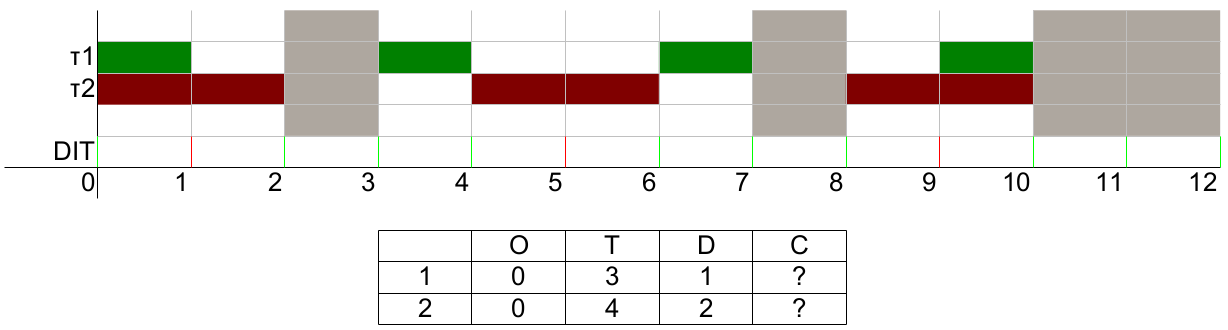
\includegraphics[width=\textwidth]{figs/dit_example.png}
\caption{The block of colors represents the arrival time and deadline of a job. DITs are represented by a green line below}
\label{fig:ditExample}
\end{center}
\end{figure}

While the definition is applicable to both synchronous and asynchronous tasks system, the following only consider the synchronous case (which is the worst-case for non-concrete tasks). The difficulties arising with asynchronous tasks are described in a later section.\\

In the synchronous case, $t=0$ and $t=H$ are DITs but there might be others in-between. The following notion is thus defined:

\begin{definition}
The earliest DIT occurring in the system strictly after $t=0$ is called the \textbf{first DIT} and is noted $t_d$.
\end{definition}

If the first DIT is $H$, then the only DITs of the system are multiple of $H$ as the occurrence of DITs is periodic.\\

The following section explains the methods to determine the value of the first DIT. Then section \ref{sct:ditsynchfeastest} will explain a method to reduce the complexity of the DBF feasibility test if the first DIT occurs before $H$.

\subsection{Existence and value}

In synchronous systems, $H$ is always a DIT, so the first DIT $t_d$ exists and is such that $t_d \leq H$. In the constrained deadline case ($D_i \leq T_i \; \forall i$), it is possible that other DITs occur before it, in which case $t_d < H$.\\

The problem of the existence of a DIT can be written with modular equations as
$$
\exists ? \; t_d \; s.t. \; \forall i : \exists a_i \in [D_i, T_i] \; s.t. \; t_d \equiv a_i \; (mod \; T_i) \\
$$

For fixed values of $a_i$, this is a case of the Generalized Chinese Remainder Theorem (see Appendix \ref{sct:appCRT}). However, in our case, each $a_i$ can take every value in the interval $[D_i, T_i]$. Observe that the particular case $a_1 \cdots a_n = 0 \cdots 0$ is always a solution, which confirm the previous result that both 0 and $H$ are always DIT.\\

If the value returned by the Chinese Remainder Theorem with a particular set of $a_i$ values is called $t_{idle} (a_1, \cdots, a_n)$\footnote{If the values are such that there are no solution, we set $t_{idle}$ to $\infty$}, the first DIT is given by $$t_d = \operatorname*{min}_{a_i \in [D_i, T_i], \; i = 1 \cdots n} t_{idle} (a_1, \cdots, a_n)$$ which require to consider a number of combinations which is exponential in the number of tasks.

\subsection{Feasibility test}
\label{sct:ditsynchfeastest}

\begin{theorem}
 Let $t_1$ be a DIT, it is sufficient to check the DBF condition at job deadlines in the interval $[0, t_1]$ to determine feasibility.
\end{theorem}

\begin{proof}
Let $t_1$ be any DIT of a synchronous task set such that $\forall t \leq t_1 : \dbf{t} \leq t$. We want to show that $\forall t > t_1 : \dbf{t} \leq t$.\\

As we are in the synchronous case, $t=0$ is a critical instant, which mean we have the earliest next job deadline for each task. Thus the DBF increase faster than in any other configuration of arrival times.\\

A DIT for some task set is similar (w.r.t. the increase of the DBF) to the initial time of the same system in the asynchronous case. In other words, after the DIT, the increase of the DBF will be slower than it was at the initial time. Which gives us, with $t_1$ being the DIT:
$$\forall t > t_1 : \dbf{t} \leq \dbf{t_1} + \dbf{t-t_1}$$

~\\

We now prove by induction that $\dbf{t-t_1} \leq t - t_1$.\\

\emph{Initial case} : We consider $t = t_1 + 1$. Thus, $\dbf{t-t_1} = \dbf{t_1 + 1 - t_1} = \dbf{1}$. As $1 \leq t_1$, we know that $\dbf{1} \leq 1$.\\

\emph{Inductive case} : We consider any $t > t_1 + 1$ and we suppose that $\forall t' < t : \dbf{t'} \leq t'$. Then, we have $\dbf{t - t_1} \leq t - t_1$ as $t - t_1 < t$.\\

And thus we have that $\dbf{t-t_1} \leq t - t_1$. As we also have $\dbf{t_1} \leq t_1$, the previous inequality becomes
$$\forall t > t_1 : \dbf{t} \leq \dbf{t_1} + \dbf{t-t_1} \leq t_1 + t - t_1 = t$$
$$\iff \forall t > t_1 : \dbf{t} \leq t$$
\end{proof}

If there exists a DIT earlier than $H$, it can be used to reduce the interval used in the DBF feasibility test.

\subsection{Results in the asynchronous case}

\begin{definition}
The \textbf{first periodic DIT} is the earliest DIT to occur strictly after the arrival of at least one job of each task.
\end{definition}

Note that the first periodic DIT will be the first DIT in the synchronous case.\\

In the synchronous case, $t = H$ is always a DIT. This is no longer true in the asynchronous case. In fact, the first periodic DIT could happen at a time $t_d > H$, or there could be no first periodic DIT at all, as seen in Fig. \ref{fig:asyncNoDit}.

\begin{figure}[h]
\begin{center}
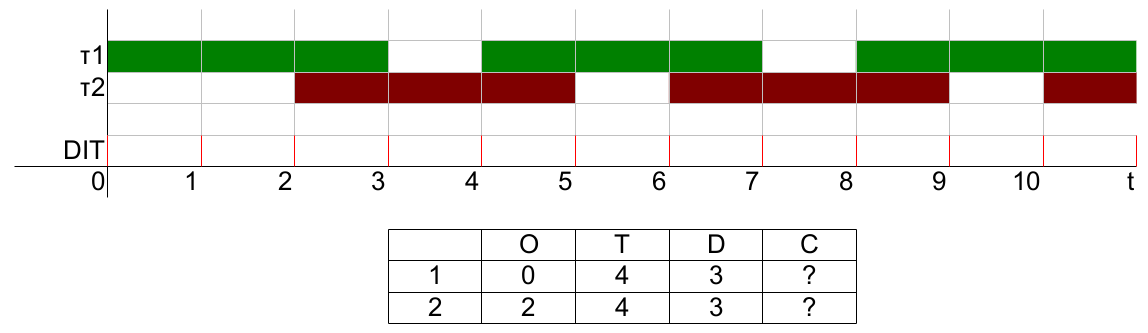
\includegraphics[width=0.75\textwidth]{figs/dit_asynchronousNoDit.png}
\caption{An asynchronous task system with no DITs after $t=0$}
\label{fig:asyncNoDit}
\end{center}
\end{figure}

\subsubsection{Existence and value}

The first periodic DIT cannot happen at a time $t > O_{max} + H$, or else it would have happened previously.\\

Similarly to the synchronous case, the problem of existence of the first periodic DIT can be written as a system of modular equation:
$$
\begin{array}{l}
	\exists ? \; t_d \; s.t. \; \forall i \; :\\
	\left\{
		\begin{array}{l}
		t_d > O_i \\
		t_d - O_i \equiv a_i \; (mod \; T_i) \\
		a_i \in [D_i, T_i]
	\end{array}
\right.
\end{array}
$$
which can, again, be solved by testing every combination of the $a_i$ and solving the corresponding equation with the Generalized Chinese Remainder Theorem. If a solution $t < O_{max}$ is found, recall that $t + k \, H, k \in \mathbb{N}$ is also a solution. Note that this time, it is possible for the system to not have any solution (e.g. Fig \ref{fig:asyncNoDit}).

\subsubsection{Feasibility test}

To understand feasibility tests in the asynchronous case, one must first understand how an asynchronous system behaves under, for example, EDF.\\

\begin{figure}[h]
$$
\begin{array}{r|c|c|c|c|l}
	 & \text{Incomplete} & \text{Transitive} & \text{Stationary} & \text{$2^{nd}$ Stationary} & \cdots \\
	 & \text{period} & \text{period} & \text{period} & \text{period} & \\
	\hline
	t & 0 & O_{max} & O_{max} + H & O_{max} + 2H & \cdots
\end{array}
$$
\begin{center}
\caption{Behavior of an asynchronous system under EDF. The value of $t$ indicates the time at which each period starts}
\label{fig:asyncBehavior}
\end{center}
\end{figure}

As shown in Fig. \ref{fig:asyncBehavior}, the system begins in the \emph{incomplete period}, where all tasks are not in the system. Then, after $O_{max}$ time units, every tasks is in the system and the \emph{transitive period} begins. Then, after $O_{max} + H$ time units, the system is faced with the same pattern of arrival as in $O_{max}$. However, because in $O_{max} + H$ every task is in the system and in $O_{max}$ some were missing, the state of the system will be different. The \emph{stationary period} then begins. It is only after $O_{max} + 2H$ time units that the system comes back into a state in which it was before.\\

For this reason, as explained in \cite{leung1982complexity}, most feasibility test for asynchronous task system (e.g. the DBF test) are restricted to the interval $[0, O_{max} + 2H]$, which has an exponential length in the number of tasks.\\

However, using DIT, we have the following property:

\begin{theorem}
Let $t_d$ be the first periodic DIT of an asynchronous system $\tau$ (supposing it exists). Then it is sufficient to check the DBF test in the interval $[0, t_d + H]$
\end{theorem}

\begin{proof}
???\\

(basically at $t_d + H$ we know that the behavior will be the same as in $t_d$)
\end{proof}

\section{Simulation}

As was shown previously, the DBF condition must be true on all instant to prove that a system is feasible. It is necessary and sufficient to check only instants where a deadline occurs, and it is also necessary and sufficient to check only instants before the hyper-period, the end of the first busy period (for constrained system only), or the first DIT. While the test itself will be shorter if the smallest of those values is used as an upper limit, the time needed to compute the value must be taken into consideration as well.\\

The DBF feasibility test was simulated on a set of synchronous system with constrained deadline. For all of those systems, the value of the hyper-period, the end of the first busy period and the first DIT is computed. Then the DBF feasibility test is applied using those upper limits. The times each methods took to complete are compared.

\subsection{Implementation model}

\subsubsection{Tasks system generation}

The method used to generate the system consisted of
\begin{itemize}
	\item Generating the $U_i$ with the \texttt{UUniSort} algorithm described in \cite{bini2005measuring}, with parameters
	\begin{itemize}
		\item $U_{tot}$ (system utilization) chosen uniformly between 0.25 and 0.75
		\item $n$ (number of tasks) chosen uniformly between 1 and 4
	\end{itemize}
	\item Generating the $T_i$ from a list of divisors (see \ref{sct:simuRemarks}). This also gives the $C_i = \lfloor U_i \, T_i \rfloor$
	\item $O_i$ (...)
	\item And finally, choosing the $D_i$ uniformly in the interval $[T_i - \frac{T_i - C_i}{e}, T_i)$, where the value of $e$ is discussed in \ref{sct:simuRemarks}.
\end{itemize}

\subsubsection{General remarks}
\label{sct:simuRemarks}
\begin{itemize}
	\item The interval used for the generation of $D_i$ can be explained by looking at the final formula for the DIT $$t_d = \operatorname*{min}_{a_i \in [D_i, T_i], \; i = 1 \cdots n} t_{idle} (a_1, \cdots, a_n)$$ The necessary number of combination of $a_i$ values to considerr is equal to the cardinality of $[D_1, T_1] \times [D_2, T_2] \times \cdots \times [D_n, T_n]$, which gives an exponential time in the number of tasks. This constraint aims to allow the DIT algorithm to terminate in an acceptable time but it also gives it a considerable advantage.
	\item The $T_i$ are not generated uniformly, but from a list of divisors of 554400\footnote{LCM of $2^5$, $3^2$, $5^2$, 7 and 11}. This prevents the value of the hyper-period from growing exponentially. Similarly, this is giving the hyper-period method an advantage.
	\item During the DBF test, the deadline are considered chronologically. The order is not important for feasible tasks set, but can change the duration of the test for unfeasible task set (where the DBF test can stop when it finds an instant where the test does not hold).
\end{itemize}

\subsubsection{Source code}

Am I allowed to make it available on GitHub? License problem with ECE?

\subsection{Results}

Fig. \ref{fig:simuTextResult} gives us the precise timing with a value of $e = 5$. While the DIT and the hyper-period methods achieve similar results, the busy period method is clearly ahead. This can be explained by the relative simplicity of its algorithm.\\

Looking more closely at the values, the trade-off offered by the DIT method compared to the hyper-period method becomes apparent. While the preprocessing time is longer for the DIT, the interval to consider for the DBF test is greatly reduced.\\

\begin{figure}[h]
\begin{center}

\begin{lstlisting}[language=]
== Test Results (on 1000 tasks system)
	Algorithms performance (upper limit computation + dbf test)
		Time with busy period: 0.02 + 0.01  =  0.03 s
		Time with DIT: 0.84 + 0.83  =  1.67 s
		Time with hyperT: 0.02 + 1.64  =  1.66 s
	Feasible? 432 , or about 43 %
\end{lstlisting}

\caption{Comparison of performance of different upper limit for the DBF feasibility test} with $e=5$
\label{fig:simuTextResult}
\end{center}
\end{figure}

~\\

Fig. \ref{fig:simuGraphE} shows the influence of the $e$ parameter, which describes the restriction imposed on the deadline parameter. Observe the exponential growth to the left. While we could think that the hyper-period curve should not be affected by $e$, this figure shows otherwise. This is explained by the fact that higher value of $e$ means more feasibility, and as was shown previously more feasibility means longer feasibility tests.

\begin{figure}[h]
\begin{center}

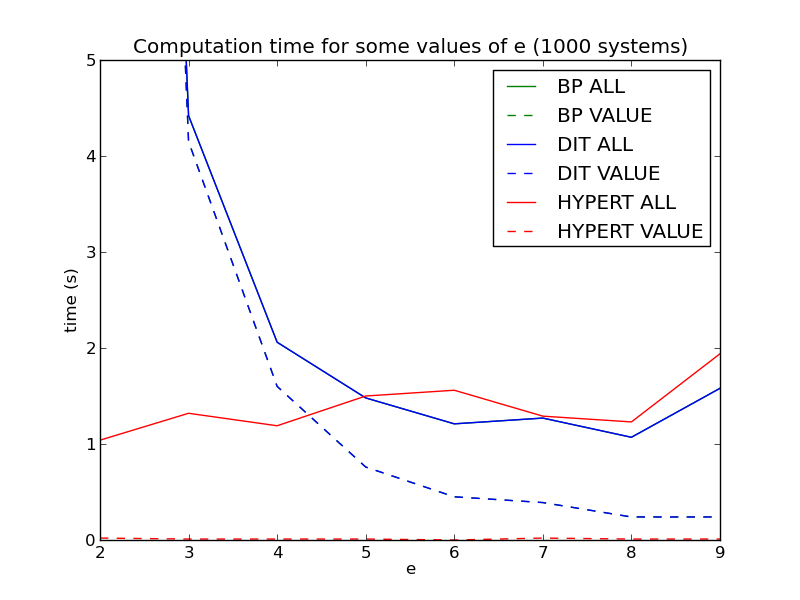
\includegraphics[width=0.75\textwidth]{figs/001_137389818886_princess.png}

\caption{Comparison of performance for different values of $e$. The plain line represent the total time, while the dotted line represent only the upper limit computation time.}
\label{fig:simuGraphE}
\end{center}
\end{figure}

\newpage
\appendix

\huge APPENDIX
\normalsize

\section{Generalized Chinese Remainder Theorem}
\label{sct:appCRT}

First let us recall the Chinese Remainder Theorem, proven in \cite{leiserson2001introduction}.

\begin{theorem}
 \textbf{Chinese Remainder Theorem} Suppose $M_1, \cdots, M_n$ are positive integers which are pairwise co-prime. Then, for any given sequence of integers $a_1, \cdots, a_n$ there exists one integer $x$ modulo $M = M_1 \cdots M_n$ solving the following system
 $$
 \left\{
	\begin{array}{llcl}
		x \equiv a_1 \; (mod \; M_1) \\
		x \equiv a_2 \; (mod \; M_2) \\
		\vdots \\
		x \equiv a_n \; (mod \; M_n)
	\end{array}
\right.
 $$

This value is given by
$$x = \sum_{i=1}^{n} a_i \frac{M}{M_i} \left[ \frac{M}{M_i} \right]_{M_i}^{-1}$$
where $[a]^{-1}_{b}$ is the modular multiplicative inverse of $a$ (mod $b$)
\end{theorem}

We can see that a requirement of the theorem is that the values of $M_i$ need to be pairwise co-prime. When this is not the case, the system is not guaranteed to have a solution. Indeed, a previous result in \cite{leiserson2001introduction} is that the system has one solution modulo $M$ if and only if $\forall \; i,j \; s.t. \; a_i \equiv a_j \; (mod \; gcd(M_i, M_j) )$ (which is clearly true when all the $M_i$ are pairwise co-prime).\\

A method to find this solution, which we will call the Generalized Chinese Remainder Theorem, is given in \cite{mathNonPairwiseCoprime}. The method consists of transforming the system into an equivalent one where the moduli are pairwise co-prime, which we can then solve using the Chinese Remainder Theorem. Another method would be the method of successive substitution.

\newpage
\nocite{*}
\bibliographystyle{plain}
\bibliography{dit-paper}


\end{document}
